\documentclass[tikz,border=2mm]{standalone}
\usepackage[scaled=0.92]{helvet}
\renewcommand{\familydefault}{\sfdefault}
\usepackage{tikz}
\usetikzlibrary{arrows.meta,calc,fit,positioning}

\definecolor{dev}{HTML}{3B6EA8}
\definecolor{devlight}{HTML}{EAF2F8}
\definecolor{clinical}{HTML}{238C7E}
\definecolor{clinicallight}{HTML}{E8F5F2}
\definecolor{analysis}{HTML}{755AA8}
\definecolor{analysislight}{HTML}{F1ECF8}
\definecolor{warm}{HTML}{C7653D}
\definecolor{warmlight}{HTML}{FAEEE8}
\definecolor{ink}{HTML}{24313D}
\definecolor{muted}{HTML}{5F6B75}
\definecolor{rule}{HTML}{B8C1C8}

\begin{document}
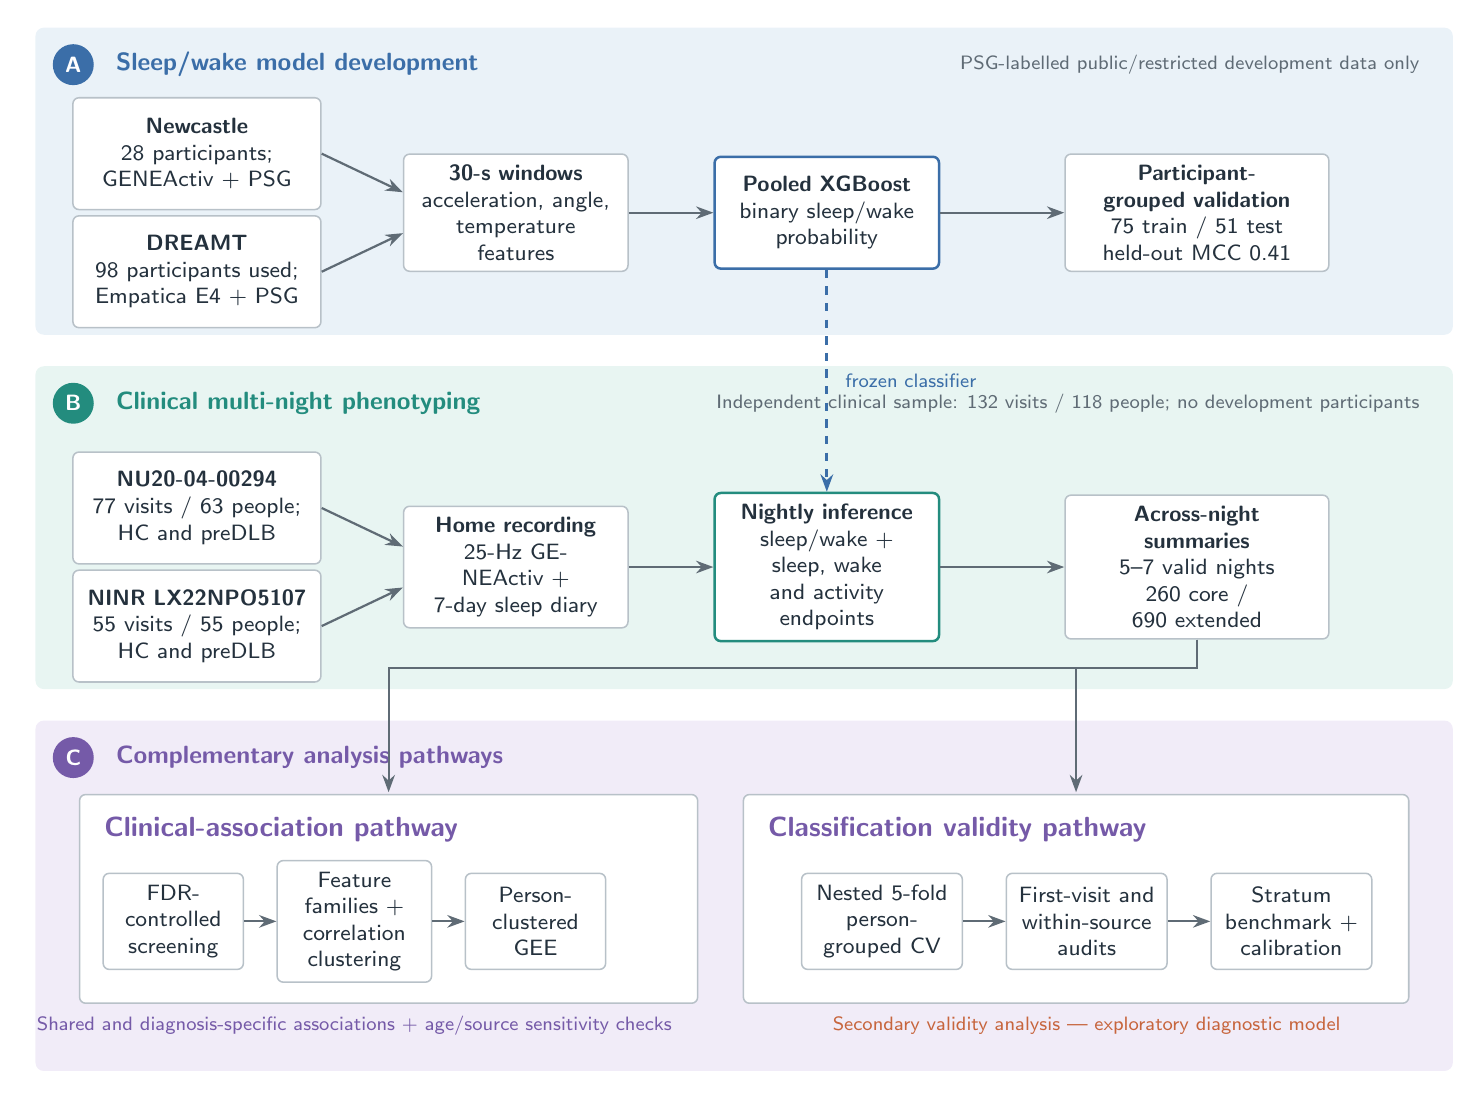
\begin{tikzpicture}[
  x=1cm,y=1cm,
  font=\fontsize{8.2}{9.6}\selectfont,
  text=ink,
  box/.style={draw=rule, line width=0.55pt, rounded corners=2.2pt,
    fill=white, align=center, inner sep=4pt, minimum height=1.42cm},
  source/.style={box, minimum width=3.15cm, text width=2.80cm},
  process/.style={box, minimum width=2.85cm, text width=2.50cm},
  result/.style={box, minimum width=3.35cm, text width=3.00cm},
  flow/.style={-{Stealth[length=2.2mm,width=1.6mm]}, line width=0.8pt, draw=muted},
  dependency/.style={-{Stealth[length=2.2mm,width=1.6mm]}, line width=1.0pt,
    draw=dev, dashed},
  paneltitle/.style={font=\bfseries\fontsize{9.2}{10.5}\selectfont, anchor=west},
  note/.style={font=\fontsize{7.2}{8.4}\selectfont, text=muted, align=center},
  tag/.style={circle, minimum size=5.2mm, inner sep=0pt, text=white,
    font=\bfseries\fontsize{8.4}{9}\selectfont}
]

% Panel backgrounds
\fill[devlight, rounded corners=3pt] (0,9.35) rectangle (18.0,13.25);
\fill[clinicallight, rounded corners=3pt] (0,4.85) rectangle (18.0,8.95);
\fill[analysislight, rounded corners=3pt] (0,0) rectangle (18.0,4.45);

% Panel A: development
\node[tag, fill=dev] at (0.48,12.78) {A};
\node[paneltitle, text=dev] at (0.90,12.78) {Sleep/wake model development};
\node[note, anchor=east] at (17.70,12.78) {PSG-labelled public/restricted development data only};

\node[source] (newcastle) at (2.05,11.65) {\textbf{Newcastle}\\28 participants; GENEActiv + PSG};
\node[source] (dreamt) at (2.05,10.15) {\textbf{DREAMT}\\98 participants used; Empatica E4 + PSG};
\node[process] (windows) at (6.10,10.90) {\textbf{30-s windows}\\acceleration, angle,\\temperature features};
\node[process, draw=dev, line width=0.9pt] (model) at (10.05,10.90) {\textbf{Pooled XGBoost}\\binary sleep/wake\\probability};
\node[result] (validation) at (14.75,10.90) {\textbf{Participant-grouped validation}\\75 train / 51 test\\held-out MCC 0.41};

\draw[flow] (newcastle.east) -- ($(windows.west)+(0,0.26)$);
\draw[flow] (dreamt.east) -- ($(windows.west)+(0,-0.26)$);
\draw[flow] (windows.east) -- (model.west);
\draw[flow] (model.east) -- (validation.west);

% Panel B: clinical phenotyping
\node[tag, fill=clinical] at (0.48,8.48) {B};
\node[paneltitle, text=clinical] at (0.90,8.48) {Clinical multi-night phenotyping};
\node[note, anchor=east] at (17.70,8.48) {Independent clinical sample: 132 visits / 118 people; no development participants};

\node[source] (nu20) at (2.05,7.15) {\textbf{NU20-04-00294}\\77 visits / 63 people; HC and preDLB};
\node[source] (ninr) at (2.05,5.65) {\textbf{NINR LX22NPO5107}\\55 visits / 55 people; HC and preDLB};
\node[process] (recording) at (6.10,6.40) {\textbf{Home recording}\\25-Hz GENEActiv +\\7-day sleep diary};
\node[process, draw=clinical, line width=0.9pt] (inference) at (10.05,6.40) {\textbf{Nightly inference}\\sleep/wake + sleep, wake\\and activity endpoints};
\node[result] (features) at (14.75,6.40) {\textbf{Across-night summaries}\\5--7 valid nights\\260 core / 690 extended};

\draw[flow] (nu20.east) -- ($(recording.west)+(0,0.26)$);
\draw[flow] (ninr.east) -- ($(recording.west)+(0,-0.26)$);
\draw[flow] (recording.east) -- (inference.west);
\draw[flow] (inference.east) -- (features.west);
\draw[dependency] (model.south) -- node[right, note, text=dev, xshift=1mm] {frozen classifier} (inference.north);

% Panel C: analysis
\node[tag, fill=analysis] at (0.48,3.98) {C};
\node[paneltitle, text=analysis] at (0.90,3.98) {Complementary analysis pathways};

\node[box, minimum width=7.85cm, text width=7.35cm, minimum height=2.65cm,
  anchor=north west] (assoc) at (0.55,3.52) {};
\node[font=\bfseries, text=analysis, anchor=north west] at ($(assoc.north west)+(0.20,-0.18)$)
  {Clinical-association pathway};
\node[process, minimum width=1.72cm, text width=1.50cm, minimum height=1.22cm]
  (screen) at (1.75,1.90) {FDR-controlled\\screening};
\node[process, minimum width=1.92cm, text width=1.68cm, minimum height=1.22cm]
  (reduce) at (4.05,1.90) {Feature families +\\correlation clustering};
\node[process, minimum width=1.72cm, text width=1.50cm, minimum height=1.22cm]
  (gee) at (6.35,1.90) {Person-clustered\\GEE};
\draw[flow] (screen.east) -- (reduce.west);
\draw[flow] (reduce.east) -- (gee.west);
\node[note, text=analysis] at (4.05,0.58) {Shared and diagnosis-specific associations + age/source sensitivity checks};

\node[box, minimum width=8.45cm, text width=7.95cm, minimum height=2.65cm,
  anchor=north east] (class) at (17.45,3.52) {};
\node[font=\bfseries, text=analysis, anchor=north west] at ($(class.north west)+(0.20,-0.18)$)
  {Classification validity pathway};
\node[process, minimum width=2.02cm, text width=1.76cm, minimum height=1.22cm]
  (nested) at (10.75,1.90) {Nested 5-fold\\person-grouped CV};
\node[process, minimum width=2.02cm, text width=1.76cm, minimum height=1.22cm]
  (audits) at (13.35,1.90) {First-visit and\\within-source audits};
\node[process, minimum width=2.02cm, text width=1.76cm, minimum height=1.22cm]
  (benchmark) at (15.95,1.90) {Stratum benchmark +\\calibration};
\draw[flow] (nested.east) -- (audits.west);
\draw[flow] (audits.east) -- (benchmark.west);
\node[note, text=warm] at (13.35,0.58) {Secondary validity analysis --- exploratory diagnostic model};

\draw[flow] (features.south) -- ++(0,-0.36) -| ($(assoc.north)+(0,0.02)$);
\draw[flow] (features.south) -- ++(0,-0.36) -| ($(class.north)+(0,0.02)$);

\end{tikzpicture}
\end{document}
